\chapter{RESULTADOS E DISCUSS�O}
Os algoritmos de ru�do de perlin, e fractal plasma foram implementados, bem como a leitura de imagens representando mapas de altura. Para uma melhor visualiza��o, o arcabou�o possui uma movimenta��o b�sica com o mouse e teclado.


As Figuras \ref{fig:tela2} e \ref{fig:tela3}, e \ref{fig:tela6} e \ref{fig:tela7} mostram os terrenos gerados variando o n�mero de itera��es do ru�do de Perlin e o n�mero de terrenos vizinhos exibidos.

\begin{figure}[H]
	\center{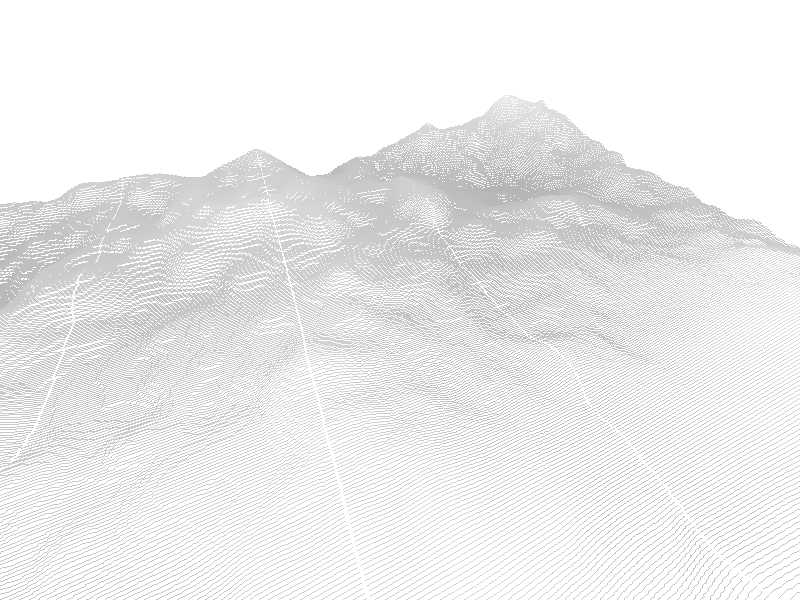
\includegraphics[width=0.5\linewidth]{img/caps/2.png}}
	\caption{\label{fig:tela2} Tela com o terreno gerado.}
\end{figure}

\begin{figure}[H]
	\center{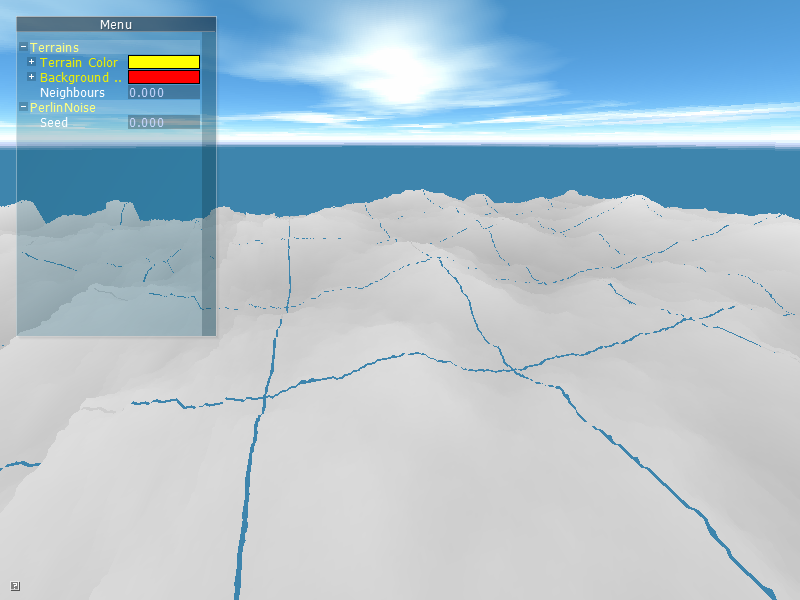
\includegraphics[width=0.5\linewidth]{img/caps/3.png}}
	\caption{\label{fig:tela3} Tela com o terreno gerado (exibi��o em \emph{wireframes}).}
\end{figure}

\begin{figure}[H]
	\center{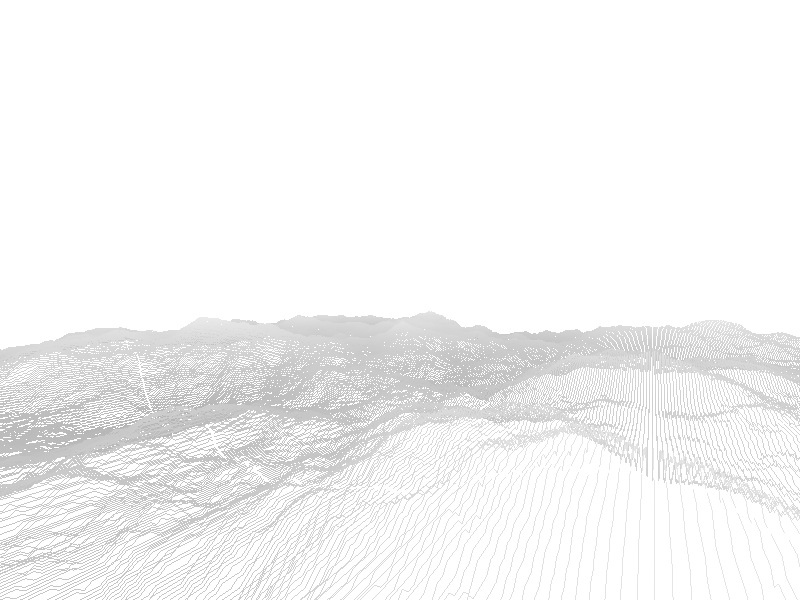
\includegraphics[width=0.5\linewidth]{img/caps/6.png}}
	\caption{\label{fig:tela6} Tela com o terreno gerado.}
\end{figure}

\begin{figure}[H]
	\center{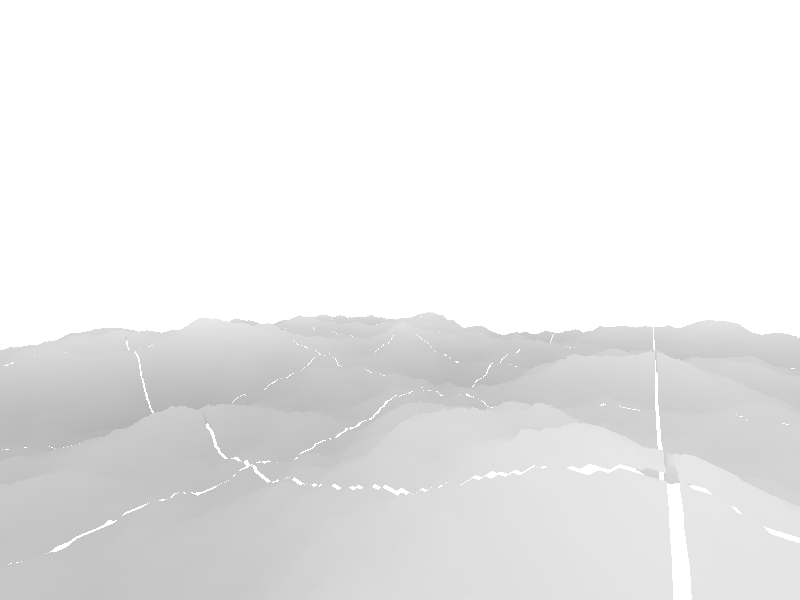
\includegraphics[width=0.5\linewidth]{img/caps/7.png}}
	\caption{\label{fig:tela7} Tela com o terreno gerado (exibi��o em \emph{wireframes}).}
\end{figure}

As Figuras \ref{fig:tela4} e \ref{fig:tela5} mostram um terreno gerado proceduralmente e o mapa de altura exibido na Figura \ref{fig:mapaaltura} inserido no arcabou�o (mostrado no arcabou�o em um tom cinza mais escuro).

\begin{figure}[H]
	\center{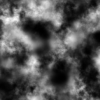
\includegraphics[width=0.25\linewidth]{img/heightmap.png}}
	\caption{\label{fig:mapaaltura} Mapa de altura.}
\end{figure}

\begin{figure}[H]
	\center{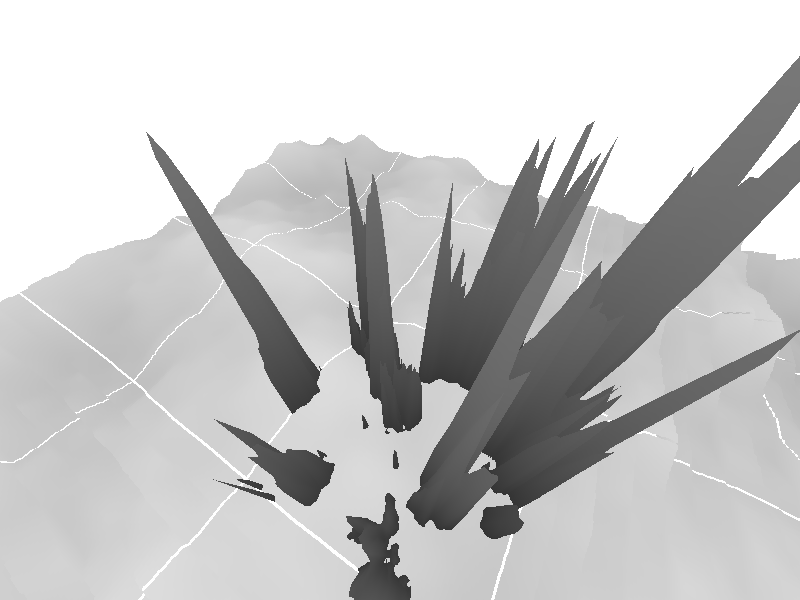
\includegraphics[width=0.5\linewidth]{img/caps/4.png}}
	\caption{\label{fig:tela4} Tela com o terreno gerado e um mapa de altura inserido.}
\end{figure}

\begin{figure}[H]
	\center{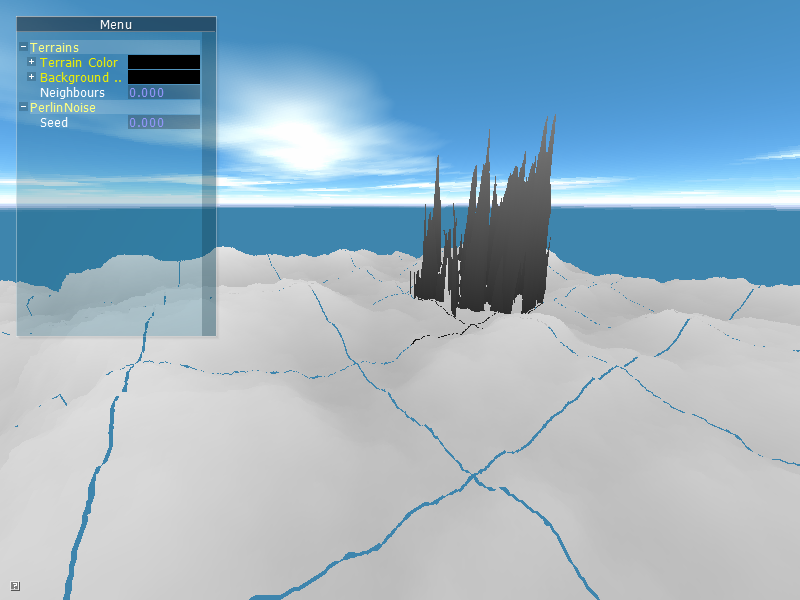
\includegraphics[width=0.5\linewidth]{img/caps/5.png}}
	\caption{\label{fig:tela5} Tela com o terreno gerado e um mapa de altura inserido (exibi��o em \emph{wireframes}).}
\end{figure}


Alguns testes foram feitos, para avaliar a varia��o de frames por segundo (\sigla{FPS}{Frames por segundo}) com a altera��o de alguns par�metros. Eles foram executados em um \emph{Athlon64 3500}, com 2GB de mem�ria \emph{RAM} e placa de v�deo GeForce6600 com 64MB de mem�ria, e consistiam em um v�o da c�mera pelo terreno durante 60 segundos, em um trajeto constante para todos os testes.


O primeiro teste (Figura \ref{fig:teste1}) mostra o impacto na mudan�a do n�mero de \emph{octaves}, considerando o n�mero de terrenos vizinhos fixo em 2. As quedas abruptas de rendimento significam momentos em que a gera��o dos novos terrenos est� acontecendo. Quanto maior o n�mero de \emph{octaves}, maior o n�mero de v�rtices da malha do terreno; explicando assim o FPS menor.

\begin{figure}[H]
	\center{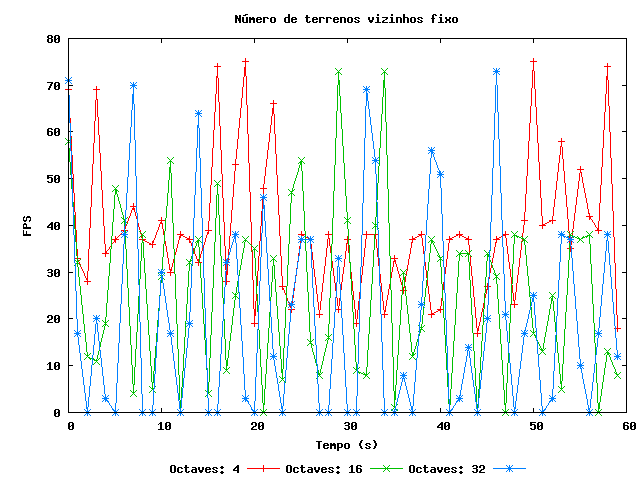
\includegraphics[width=0.5\linewidth]{img/graficos/teste1/teste1.png}}
	\caption{\label{fig:teste1} Teste variando o n�mero de \emph{octaves}, e o n�mero de terrenos vizinhos fixo em 2.}
\end{figure}

O segundo teste (Figura \ref{fig:teste2}) mostra o impacto variando o n�mero de terrenos vizinhos. Como era de se esperar, quanto maior o n�mero de vizinhos, menor o FPS.

\begin{figure}[H]
	\center{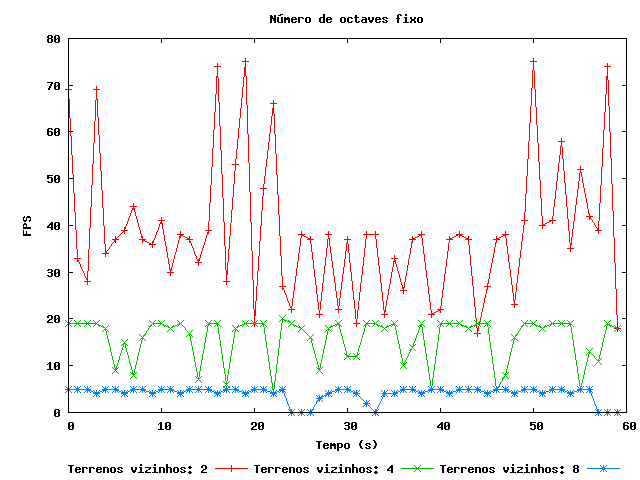
\includegraphics[width=0.5\linewidth]{img/graficos/teste2/teste2.png}}
	\caption{\label{fig:teste2} Teste variando o n�mero de terrenos vizinhos, e o n�mero de octaves fixo.}
\end{figure}